\chapter{The Governing Equations}
The semi-geostrophic equations first introduced by \cite{Eliassen1962}
form the basis of our model for frontogenesis. Widely noted to be more rigorous than the classical quasi-geostrophic equations in their description of the formation of weather fronts 
\cite{Cullen2006a, Hoskins1975}. 
In this chapter a summary of key steps that lead to the Eady model for frontogensis that was developed by Hoskins and Bretherton , 1972, \cite{Hoskins1972} is given. Based on the model for baroclinic instability proposed by Eady, 1949, incorporating a linear stratification in density and a constant vertical shear in the horizontal velocity component. A co-ordinate transform to geostrophic co-ordinates by  \cite{Hoskins1975} 
facilitates the numerical implementation of these equations and subsequent interpretation of results. For the following the main points are summarised from Cullen 2006 \cite{Cullen2006a} in formulating the model to be implemented numerically.
\section{The Semi-Geostrophic Equations \label{SGeqns}} 
\subsection{The 3D Incompressible Boussinesq Equations}
\begin{figure}[h]	
	\centering
	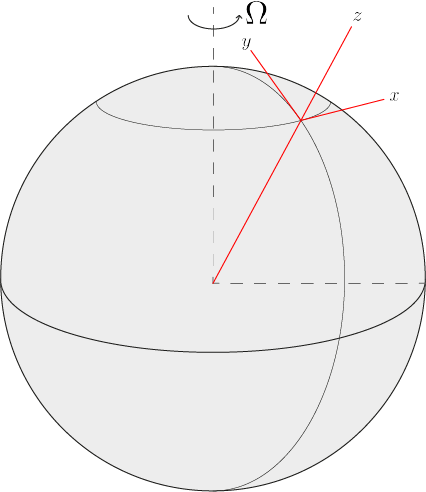
\includegraphics[width=5cm]{background/local_cartesian}
	\caption{Local cartesian co-ordinates $\left(x,y,z\right)$ on Earth}
	\label{fig:localcartesian}
\end{figure}
We begin with the $3$D incompressible Boussinesq equations \ref{3DBous} to describe atmospheric flow. Adopting cartesian co-ordinates $\left(x,y,z\right)$ representing the zonal, meridional and radial directions on the Earth respectively, as shown in \ref{fig:localcartesian}. The corresponding velocity components are $\bm{u}=\left(u,v,w\right)$, with $\rho_0$ representing the constant density and $p$ denoting the pressure.
\begin{equation}
	\begin{aligned}
		\frac{\mathrm{D}u}{\mathrm{D}t}	- fv  &= -\frac{1}{\rho_0}\frac{\partial p}{\partial x}\\
		\frac{\mathrm{D}v}{\mathrm{D}t}	+ fu  &= -\frac{1}{\rho_0}\frac{\partial p}{\partial y}\\
		\frac{\mathrm{D}w}{\mathrm{D}t} &= -\frac{1}{\rho_0}\frac{\partial p}{\partial z} + b\\
		\frac{\mathrm{D} b}{\mathrm{D}t} &= 0\\
		\nabla \cdot \bm{u} &= 0
	\end{aligned}
\label{3DBous}
\end{equation}
Under the Boussinesq assumption that density fluctuations are small, the thermodynamic equation is written as equation (4) in the system above. The buoyancy is characterised by Potential Temperature, $\theta$ as $b = \frac{g\theta}{\theta_0}$. By also introducing the geopotential $\phi = \frac{p}{\rho_0}$, equations \ref{3DBous} are rewritten as
\begin{equation}
	\begin{aligned}
		\frac{\mathrm{D}u}{\mathrm{D}t}	- fv  &= -\frac{\partial \phi}{\partial x}\\
		\frac{\mathrm{D}v}{\mathrm{D}t}	+ fu  &= -\frac{\partial \phi}{\partial y}\\
		\frac{\mathrm{D}w}{\mathrm{D}t} &= -\frac{\partial \phi}{\partial z} + \frac{g\theta}{\theta_0}\\
		\frac{\mathrm{D} \theta}{\mathrm{D}t} &= 0\\
		\nabla \cdot \bm{u} &= 0
	\end{aligned}
\label{3DBousPT}
\end{equation}
where $\theta_0$ and $g$ denote initial potential temperature and acceleration due to gravity respectively. \\
$\frac{\mathrm{D}}{\mathrm{D}t} \equiv \frac{\partial}{\partial t} + u\frac{\partial}{\partial x} + v\frac{\partial}{\partial y} + w\frac{\partial}{\partial z},\qquad$ 
$\nabla \equiv \left(\frac{\partial}{\partial x}, \frac{\partial}{\partial y},\frac{\partial}{\partial z}\right)$
\subsection{The Vertical Slice Model}
To facilitate the study of frontogenesis a vertical slice model is introduced. In this report the vertical slice is defined as the $\left(x-z\right)$ plane. Perturbations to the leading-order fields are considered as functions of $x,z$ and $t$ only, whereas the leading order terms in $\theta$ and $\phi$ are functions of $\left(y,z\right)$. Retaining the potential temperature gradient normal to the slice is crucial to the subsequent evolution of the front. Following the ideas of Yamazaki, 2017 \cite{Yamazaki2017} we introduce,
\begin{equation}
	\begin{aligned}
		\theta = \bar{\theta}(y,z) + \theta'(x,z,t)\\ 
		\phi = \bar{\phi}(y,z) + \varphi(x,z,t)
	\end{aligned}
\end{equation}
With the background fields chosen as,
\begin{equation}
	\begin{aligned}
		\bar{\theta} &= -Cy + \frac{N^2\theta_0z}{g}\\ 
		\frac{\partial \bar{\phi}}{\partial y} &= -\frac{Cg}{\theta_0}\left(z - H/2\right)
	\end{aligned}
\label{bgTP}
\end{equation}
The Brunt-V\"{a}is\"{a}l\"{a} frequency $N^2 = \frac{g}{\theta_0}\frac{\partial \theta}{\partial z}$ characterises the stratification of density in the slice and $H$ denotes the vertical height of the domain. The constant, normal potential temperature gradient, $\frac{\partial \theta}{\partial y} = -C$.\\
\linebreak
If the hydrostatic approximation $\frac{\mathrm{D}w}{\mathrm{D}t} = 0$ is made in addition, then the third momentum equations gives,
\begin{equation}
\frac{\partial \bar{\phi}}{\partial z} = -\frac{Cgy}{\theta_0} + N^2z\\
\label{bgP}
\end{equation}
To reach the vertical slice model we substitute $\theta = \bar{\theta} + \theta'$ and $\phi = \bar{\phi} + \varphi$ with expressions \ref{bgTP} and \ref{bgP} into equations \ref{3DBousPT}. 
\begin{equation}
	\begin{aligned}
		\frac{\mathrm{D}u}{\mathrm{D}t}	- fv  &= -\frac{\partial}{\partial x}\left(\bar{\phi} + \varphi\right)
		\\
		\frac{\mathrm{D}v}{\mathrm{D}t}	+ fu  &= -\frac{\partial}{\partial y}\left(\bar{\phi} + \varphi\right)
		\\
		0 &=\frac{\partial}{\partial z}\left(\bar{\phi} + \varphi\right) - \frac{g}{\theta_0}\left(\bar{\theta} + \theta'\right)
		\\
		0 & =\frac{\partial }{\partial t}\left(\bar{\theta} + \theta'\right) +u\frac{\partial }{\partial x}\left(\bar{\theta} + \theta'\right) + v\frac{\partial }{\partial y}\left(\bar{\theta} + \theta'\right) + w\frac{\partial }{\partial z}\left(\bar{\theta} + \theta'\right)
		\\
		0 &= \frac{\partial u}{\partial x} + \frac{\partial v}{\partial y} + \frac{\partial w}{\partial z}
	\end{aligned}
\end{equation}
By neglecting $\partial/\partial y$ terms in perturbation variables after rearrangement 
\begin{equation}
	\begin{aligned}
		\frac{\mathrm{D}u}{\mathrm{D}t}	- fv  &= -\frac{\partial \varphi}{\partial x}
		\\
		\frac{\mathrm{D}v}{\mathrm{D}t}	+ fu  &= -\frac{\partial \varphi}{\partial y} + \frac{Cg}{\theta_0}\left(z - H/2\right)
		\\
		0 &=\frac{\partial \varphi}{\partial z} - \frac{g\theta'}{\theta_0}
		\\
		0 & =\frac{\partial \theta'}{\partial t} +u\frac{\partial \theta'}{\partial x} - Cv + w\frac{\partial \theta'}{\partial z} + w\frac{N^2\theta_0}{g}
		\\
		0 &= \frac{\partial u}{\partial x} + \frac{\partial w}{\partial z}
	\end{aligned}
\label{VerticalSlice}
\end{equation}
\comments{$w\frac{N^2\theta_0}{g}$ shouldn't be there !}
\subsection{The Geostrophic Momentum Approximation}
To reach the final semi-geostrophic Eady model for frontogenesis the Geostrophic Momentum approximation is made. Developed by Hoskins, 1975 \cite{Hoskins1975}, where further detail can be found, the following section gives a brief summary of the key arguments.\\
\linebreak
Going back to equations \ref{3DBousPT}. We consider an expansion in the Rossby number $\epsilon = U/fL$ where $U$ and $L$ are horizontal velocity and length scaled respectively. Expanding the momentum equations in \ref{3DBousPT} in leading-order (geostrophic) and first order (ageostrophic) terms in $\epsilon$, so that,
\begin{equation*}
	\bm{u} = \bm{u_g} + \epsilon \bm{u_a} \qquad \phi = \phi_g +\epsilon \phi_a
\end{equation*}
Acceleration terms are found to be $O(\epsilon)$ so that at the leading order the geostrophic balance is found to be,
\begin{equation}
	fv_g  = -\frac{\partial \phi_g}{\partial x} \qquad
	-fu_g  = -\frac{\partial \phi_g}{\partial y}
\end{equation}
Subsequent analysis as detailed in Hoskins 1975, \cite{Hoskins1975} finds the prognostic equations for ageostrophic variables to be such that the momentum $\frac{\mathrm{D}u}{\mathrm{D}t}, \frac{\mathrm{D}v}{\mathrm{D}t}$ are replaced with their geostrophic counterparts $\frac{\mathrm{D}u_g}{\mathrm{D}t}, \frac{\mathrm{D}v_g}{\mathrm{D}t}$. Noting that in the vertical slice model $u_g = 0$ we find equations \ref{VerticalSlice} with the geostrophic momentum approximation as
\begin{equation}
	\begin{aligned}
		-fv_g + \frac{\partial \varphi}{\partial x} = 0,\\
		\frac{Dv_g}{Dt} + fu -\frac{Cg}{\theta _0}\left(z-H/2\right) = 0,\\
		\frac{D\theta'}{Dt} - Cv_g = 0,\\
		\frac{\partial \varphi}{\partial z} - g\frac{\theta'}{\theta_0} = 0,\\
		\nabla \cdot \bm{u} = 0.
	\end{aligned}
\label{EadyModel}
\end{equation}
\comments{First equation is different - $-fv_g$ isn't $O(\epsilon)$??}
Where, for convenience the subscript a has been dropped. With,\\
$\frac{\mathrm{D}}{\mathrm{D}t} \equiv \frac{\partial}{\partial t} + u\frac{\partial}{\partial x} + w\frac{\partial}{\partial z},\qquad$ 
$\nabla \equiv \left(\frac{\partial}{\partial x},\frac{\partial}{\partial z}\right)$\\
\linebreak
The corresponding energy integral is,
\begin{equation}
	E = \iint \frac{1}{2}v_g^2 - \frac{g\theta'}{\theta_0}\left(z - H/2\right)\textrm{d}x\textrm{d}z
\end{equation}
Equations \ref{EadyModel} form the basis of the subsequent investigation of frontogenesis in this report. They are to be solved over the domain $\Gamma = [-L,L] \times [0,H]$, with the periodic boundary conditions in $x$ and the rigid-lid boundary condition $w = 0$ on $z = 0,H$. The baroclinic instability introduced from Cullen 2006 \cite{Cullen2006a} in the form of a perturbation to $\theta'$, 
\begin{equation}
	\theta' = \frac{N^2\theta_0 z}{g} + B\sin\left(\pi\left(x/L + z/H\right)\right)
\end{equation}
\begin{itemize}
	\item \textbf{Key Scalings}
	It is worth noting that Eady's original model for baroclinic instability was developed under a quasi-geostrophic model, where $\epsilon = Fr \ll 1$ in contrastsemi-geostrophic theory the assumes, $\epsilon \ll 1$ with $\epsilon < Fr$.
\end{itemize}
\comments{does this need including?}
\section{Transformation to Geostrophic Co-ordinates \label{transformation}}
To facilitate the implementation of the numerical scheme we will subsequently use to solve equations \ref{EadyModel} a \textquotedblleft geostrophic co-ordinate\textquotedblright system first introduced by Hoskins \cite{Hoskins1975} in the horizontal directions $(x,y)$. The geostrophic co-ordinates describe the position of particles had they evolved under their geostrophic velocity. The transformation was later developed by Cullen \cite{Cullen2006a} to include a transformation in terms of $\theta '$ in the vertical direction.
\begin{equation}
	X = x + \frac{v_g}{f}, \qquad Z = \frac{g\theta'}{f^2\theta_0}
\end{equation}
By defining
\begin{equation}
P = \frac{1}{2}x^2 + \frac{1}{f^2}\varphi
\label{P}
\end{equation}
It is clear that,
\begin{equation*}
	\begin{aligned}
		\nabla P &= \left(x + \frac{1}{f^2}\frac{\partial \varphi}{\partial x}, \frac{1}{f^2} \frac{\partial \theta'}{\partial z}\right)
		&= \left(x + \frac{v_g}{f}, \frac{g\theta'}{f^2\theta_0}\right)
	\end{aligned}
\end{equation*}
So that upon substitution from the first and fourth equations in \ref{EadyModel} we find,
\begin{equation}
	\nabla P = (X,Z)
\label{gradP}
\end{equation}
By noting that,
\begin{equation*}
\frac{\mathrm{D}X}{\mathrm{D}t} = \frac{\mathrm{D}x}{\mathrm{D}t} + \frac{1}{f}\frac{\mathrm{D}v_g}{\mathrm{D}t} = u + \frac{1}{f}\frac{\mathrm{D}v_g}{\mathrm{D}t}, \qquad \frac{\mathrm{D}Z}{\mathrm{D}t} = \frac{g}{f^2\theta_0} \frac{\mathrm{D}\theta '}{\mathrm{D}t}
\end{equation*}
the momentum equations from \ref{EadyModel} are transformed into geostrophic co-ordinates as
\begin{equation}
		\frac{\mathrm{D}X}{\mathrm{D}t} -\frac{Cg}{f\theta _0}\left(z-H/2\right) = 0,\qquad
		\frac{\mathrm{D}Z}{\mathrm{D}t} - \frac{Cg}{f\theta_0}\left(X - x\right) = 0,
\label{Gmom}
\end{equation}
It is also shown in \cite{Cullen2006a} that the continuity equation holds in geostrophic co-ordinates. with $\bm{U} = \frac{Cg}{f\theta _0}\left(X-x,z-H/2\right) $
Putting together equations \ref{P}, \ref{gradP}, \ref{Gmom} the Eady Model in geostrophic co-ordinates is 
\begin{equation}
	\begin{aligned}
		\frac{\mathrm{D}X}{\mathrm{D}t} -\frac{Cg}{f\theta _0}\left(z-H/2\right) = 0 \\
		\frac{\mathrm{D}Z}{\mathrm{D}t} - \frac{Cg}{f\theta_0}\left(X - x\right) = 0,\\
		P = \frac{1}{2}x^2 + \frac{1}{f^2}\varphi,\\
		\nabla P = (X,Z)\\
		\nabla \cdot \bm{U} = 0
	\end{aligned}
\label{EadyGC}
\end{equation}
The corresponding energy integral is,
\begin{equation}
E = f^2 \iint \frac{1}{2}\left(X-x\right)^2 - Z\left(z - H/2\right)\textrm{d}x\textrm{d}z
\end{equation}
It is shown by Cullen \cite{Cullen2006a} that the system of equations above can be recast as an optimal transport problem satisfying energy minimisation with a quadratic cost,
\comments{show that the energy minimisation is equaivalent to the equation below}
\begin{equation}
E = f^2 \iint \frac{1}{2}\left(\left(X-x\right)^2 + \left(Z - z\right)^2\right)\textrm{d}x\textrm{d}z
\end{equation}